
%(BEGIN_QUESTION)
% Copyright 2010, Tony R. Kuphaldt, released under the Creative Commons Attribution License (v 1.0)
% This means you may do almost anything with this work of mine, so long as you give me proper credit

Suppose an electrician uses a {\it megger} to measure between the following test points on this three-phase 480 VAC induction motor, with the following results:

$$\includegraphics[width=15.5cm]{i02392x01.eps}$$

% No blank lines allowed between lines of an \halign structure!
% I use comments (%) instead, so that TeX doesn't choke.

$$\vbox{\offinterlineskip
\halign{\strut
\vrule \quad\hfil # \ \hfil & 
\vrule \quad\hfil # \ \hfil \vrule \cr
\noalign{\hrule}
%
% First row
{\bf Test points} & {\bf Measurement} \cr
%
\noalign{\hrule}
%
% Another row
T1 and motor frame & 325 M$\Omega$ \cr
%
\noalign{\hrule}
%
% Another row
T2 and motor frame & 325 M$\Omega$ \cr
%
\noalign{\hrule}
%
% Another row
T3 and motor frame & 325 M$\Omega$ \cr
%
\noalign{\hrule}
} % End of \halign 
}$$ % End of \vbox

What do these measurements suggest about the health of this electric motor?  If you think these measurements are normal, say so.  If not, explain what their abnormalities specifically tell you about the motor's condition.  Be as detailed as possible in your answer regarding the nature and location of the fault, if you think there is indeed something wrong with the motor.

\underbar{file i02392}
%(END_QUESTION)





%(BEGIN_ANSWER)

These are healthy measurements, as the motor's windings should not connect to ground.

%(END_ANSWER)





%(BEGIN_NOTES)

{\bf This question is intended for exams only and not worksheets!}.

%(END_NOTES)

